\section{Application 3: Sampling from Precision Matrices (e.g. for Inverse Problems)}

\gp{TODO}

\begin{figure}[t!]
  \centering
  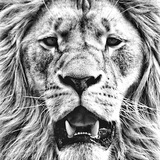
\includegraphics[width=0.24\linewidth]{figures/lion160.png}
  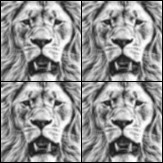
\includegraphics[width=0.24\linewidth]{figures/init_lion160.png}
  
\includegraphics[width=0.24\linewidth]{figures/posterior_lion160.png}
  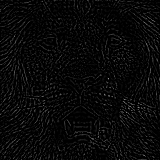
\includegraphics[width=0.24\linewidth]{figures/delta_lion160.png}
  \caption{
    Using CIQ for solving inverse problems, such as unsupervised image super-resolution.
    This requires sampling from a precision matrix of size $25,\!600$.
    ({\bf Left}) original image ($D=25,\!600$).
    ({\bf Middle Left}) Downsampled images.
    ({\bf Middle Right}) Reconstructed image.
    ({\bf Right}) Delta between original and reconstruction.
  }
  \label{fig:robotics}
\end{figure}

\gp{Time per iteration: 1.63s, avg pixel RMSE: 23.19/256, used TitanRTX}

\cite{griffin2017hierarchical}
\cite{bardsley2012mcmc}
\cite{waller1997hierarchical}
\cite{besag1991bayesian}
\cite{knorr2002block}
\cite{chipman1996bayesian}
